% ADS2 AE1 Report written in LaTeX by Inesh Bose

\documentclass{article}

%==============================================================================
%% Packages and Command Setting

\usepackage[utf8]{inputenc}
\setcounter{secnumdepth}{0}
\newcommand{\code}[1]{\texttt{#1}}
\usepackage{pgfplots}
\usepackage{geometry}
\usepackage{float}
\usepackage{hyperref}
\usepackage[symbol]{footmisc}

\hypersetup{
    colorlinks,
    citecolor=black,
    filecolor=black,
    linkcolor=black,
    urlcolor=black
}
\renewcommand{\thefootnote}{\fnsymbol{footnote}}

%==============================================================================
%% Title Page

\title{Algorithms and Data Structures \\ Assessed Exercise 1}
\author{Inesh Bose}
\date{}

\begin{document}

\maketitle
\tableofcontents

%==============================================================================
%% Part 1

\newpage

\section{Part 1}
All algorithms have similar method names and a \code{Swap()} method that is \code{public static} in order to begin the sorting. All other methods are \code{private static}.

\bigskip

\subsection{Basic Quick Sort}
The basic quick sort introduced in Lecture 5 (slide 74) has been implemented in \code{QuickSortA.java}. It includes three methods - \code{Swap(int[], int, int), Partition(int[], int, int)} and \code{Sort(int[], int, int)}. \\

\subsection{Quick Sort with Cutoff}
In this sorting technique (implemented in \code{QuickSortB.java}), subarrays with elements less than the cutoff are sorted using \code{InsertionSort} as it is more efficient for smaller arrays. For larger subarrays, the basic quick sort is used. This technique is tested through \code{SortWithCutOff(int[], int, int, int)} in \code{TimeSortingAlgorithms.java} that changes the cutoff (\code{public static}) in multiples of 5. By default, there are 4 multiples, but it can be changed when calling the method. \\

\subsection{Quick Sort using Median-of-Three}
This technique is implemented in \code{QuickSortC.java}. \code{Median(int[], int, int)} takes the first, middle and last elements of the array and sorts them. The middle element is then taken as the pivot. \\

\subsection{3-Way-Quick Sort}
\code{QuickSortD.java} implements the 3-Way-Quick Sort (based on \textit{Dutch National Flag} algorithm). \code{Partition(int[], int, int)} divides the array in 3 subarrays by comparing it to the pivot; it then returns the first and last indices of the subarray with elements equal to the pivot.

%==============================================================================
%% Part 2 : Page 1 (Introduction)

\newpage
\newgeometry{top=1in,bottom=1in}

\section{Part 2}
The sorting techniques were tested using eight files on three machines with different hardware.

\begin{table}[H]
\centering
\begin{tabular}{c|c|c}
\textbf{EliteOne} & \textbf{Envy}       & \textbf{XPS}       \\ \hline
i7-7700 @ 3.60GHz & i7-6700HQ @ 2.60GHz & i7-9750H @ 2.60GHz \\
16GB DDR3         & 16GB DDR3           & 16GB DDR4                             
\end{tabular}
\caption{details of machines}
\end{table}

\begin{table}[H]
\centering
\begin{tabular}{cc}
dutch.txt (1,916 KB): 500,000 & int10.txt (1 KB): 10             \\
int100.txt (1 KB): 100        & int500k (3,310 KB): 500,000      \\
int20k.txt (133 KB): 20,000   & int50.txt (1 KB): 50             \\
int1000.txt (4 KB): 1,000     & intBig.txt (6,619 KB): 1,000,000
\end{tabular}
\caption{details of files}
\end{table}

\bigskip

\subsection{Basic Quick Sort Graph}
In the graph, we see the variation and how size of an array affects time. However, although \code{dutch.txt} is half the size of \code{intBig.txt}, there are no duplicates therefore requiring more time. \\

\smallskip

\pgfplotsset{width=15cm,compat=1.9}
\begin{center}
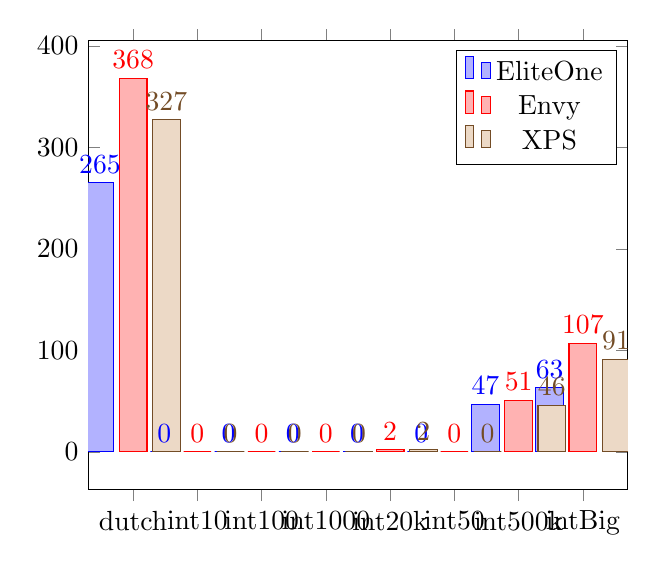
\begin{tikzpicture}
\begin{axis}[
    ybar,
    nodes near coords,
    enlargelimits,
    symbolic x coords={dutch, int10, int100, int1000, int20k, int50, int500k, intBig},
    xtick=data]
    \addplot coordinates {
        (dutch, 265)
        (int10, 0)
        (int100, 0)
        (int1000, 0)
        (int20k, 0)
        (int50, 0)
        (int500k, 47)
        (intBig, 63)
    };
    \addplot coordinates {
        (dutch, 368)
        (int10, 0)
        (int100, 0)
        (int1000, 0)
        (int20k, 2)
        (int50, 0)
        (int500k, 51)
        (intBig, 107)
    };
    \addplot coordinates {
        (dutch, 327)
        (int10, 0)
        (int100, 0)
        (int1000, 0)
        (int20k, 2)
        (int50, 0)
        (int500k, 46)
        (intBig, 91)
    };
\legend{EliteOne, Envy, XPS}
\end{axis}
\end{tikzpicture}
\end{center}

\restoregeometry

%==============================================================================
%% Part 2 : Page 2 (Quick Sort with Cutoff Graph)

\newpage
\newgeometry{top=1.0in}

\subsection{Quick Sort with Cutoff Graph}
\textbf{(Tested on Envy)} \\
\\ There are four cutoffs for each file. Subarrays with elements less than the cutoff are sorted using \code{InsertionSort}. Arrays such as \code{dutch.txt} were sorted faster with a cutoff of 10, whereas \code{intBig.txt} was slower with cutoff 10. \\
\smallskip \\

\hspace{-2.8cm}
\pgfplotsset{width=20cm,compat=1.9}
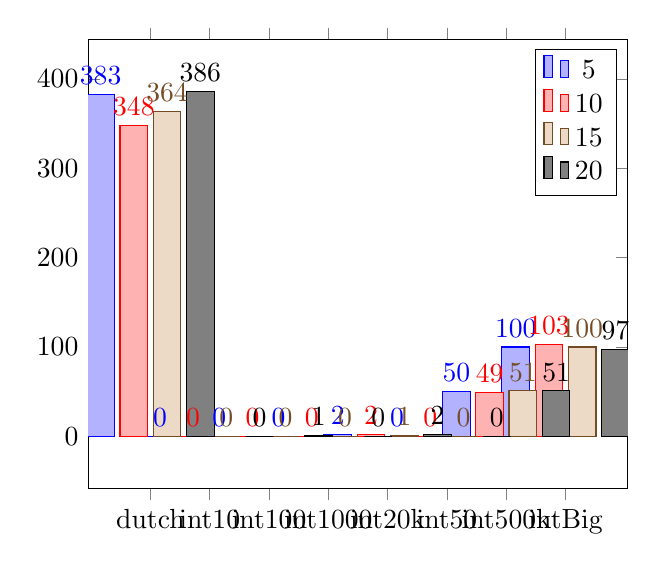
\begin{tikzpicture}
\begin{axis}[
    ybar,
    enlargelimits=0.15,
    symbolic x coords={dutch, int10, int100, int1000, int20k, int50, int500k, intBig},
    xtick=data,
    nodes near coords,
    nodes near coords align={vertical},
    ]
\addplot coordinates {(dutch,383)(int10,0)(int100,0)(int1000,0)(int20k,2)(int50,0)(int500k,50)(intBig,100)};
\addplot coordinates {(dutch,348)(int10,0)(int100,0)(int1000,0)(int20k,2)(int50,0)(int500k,49)(intBig,103)};
\addplot coordinates {(dutch,364)(int10,0)(int100,0)(int1000,0)(int20k,1)(int50,0)(int500k,51)(intBig,100)};
\addplot coordinates {(dutch,386)(int10,0)(int100,1)(int1000,0)(int20k,2)(int50,0)(int500k,51)(intBig,97)};
\legend{5, 10, 15, 20}
\end{axis}
\end{tikzpicture}

\restoregeometry

%==============================================================================
%% Part 2 : Page 3 (Quick Sort using Median-of-Three Graph)

\newpage

\subsection{Quick Sort using Median-of-Three Graph}
This graph should be similar to Basic Quick Sort Graph but slightly faster as Median-of-Three is an \textit{improvement} on the basic quick sort by choosing the pivot value. \code{dutch.txt}, however, was sorted in much faster times. This means that duplicate values can lead to slower quick sort. \\

\smallskip

\pgfplotsset{width=15cm,compat=1.9}
\begin{center}
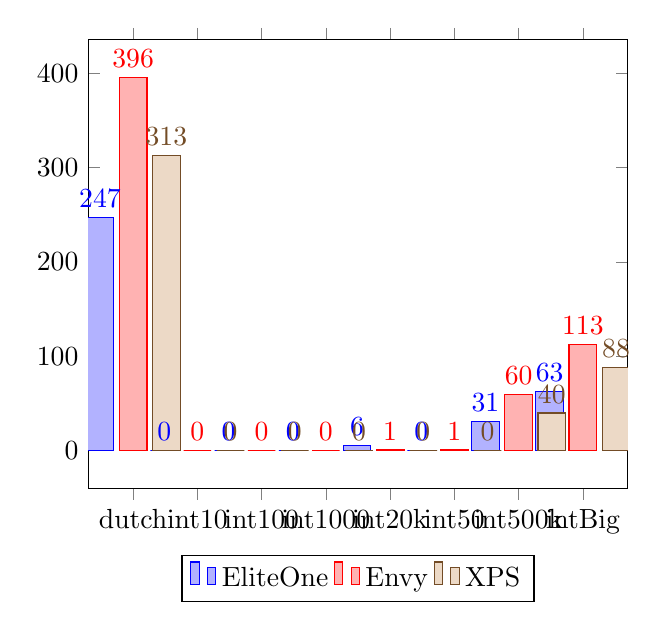
\begin{tikzpicture}
\begin{axis}[
    ybar,
    legend style={at={(0.5,-0.15)},
    anchor=north,legend columns=-1},
    nodes near coords,
    enlargelimits,
    symbolic x coords={dutch, int10, int100, int1000, int20k, int50, int500k, intBig},
    xtick=data]
    \addplot coordinates {
        (dutch, 247)
        (int10, 0)
        (int100, 0)
        (int1000, 0)
        (int20k, 6)
        (int50, 0)
        (int500k, 31)
        (intBig, 63)
    };
    \addplot coordinates {
        (dutch, 396)
        (int10, 0)
        (int100, 0)
        (int1000, 0)
        (int20k, 1)
        (int50, 1)
        (int500k, 60)
        (intBig, 113)
    };
    \addplot coordinates {
        (dutch, 313)
        (int10, 0)
        (int100, 0)
        (int1000, 0)
        (int20k, 0)
        (int50, 0)
        (int500k, 40)
        (intBig, 88)
    };
\legend{EliteOne, Envy, XPS}
\end{axis}
\end{tikzpicture}
\end{center}

%==============================================================================
%% Part 2 : Page 4 (3-Way-Quick Sort Graph)

\newpage

\subsection{3-Way-Quick Sort Graph}
Since this technique is efficient for values with duplicates, therefore \code{int500k.txt} and \code{intBig.txt} have an improvement. \\

\smallskip

\pgfplotsset{width=15cm,compat=1.9}
\begin{center}
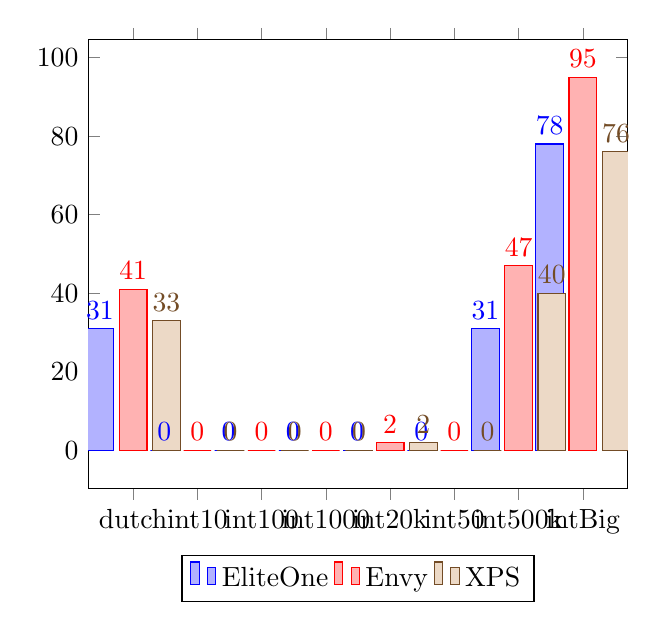
\begin{tikzpicture}
\begin{axis}[
    ybar,
    legend style={at={(0.5,-0.15)},
    anchor=north,legend columns=-1},
    nodes near coords,
    enlargelimits,
    symbolic x coords={dutch, int10, int100, int1000, int20k, int50, int500k, intBig},
    xtick=data]
    \addplot coordinates {
        (dutch, 31)
        (int10, 0)
        (int100, 0)
        (int1000, 0)
        (int20k, 0)
        (int50, 0)
        (int500k, 31)
        (intBig, 78)
    };
    \addplot coordinates {
        (dutch, 41)
        (int10, 0)
        (int100, 0)
        (int1000, 0)
        (int20k, 2)
        (int50, 0)
        (int500k, 47)
        (intBig, 95)
    };
    \addplot coordinates {
        (dutch, 33)
        (int10, 0)
        (int100, 0)
        (int1000, 0)
        (int20k, 2)
        (int50, 0)
        (int500k, 40)
        (intBig, 76)
    };
\legend{EliteOne, Envy, XPS}
\end{axis}
\end{tikzpicture}
\end{center}

%==============================================================================
%% Part 2 : Page 5 (Insertion Sort Graph)

\newpage

\subsection{Insertion Sort Graph}
Undoubtedly, sort times are incredibly high for large arrays reaching upto \textbf{102,811 milliseconds} (1.71 minutes) for \code{intBig.txt}. \\

\smallskip

\pgfplotsset{width=15cm,compat=1.9}
\begin{center}
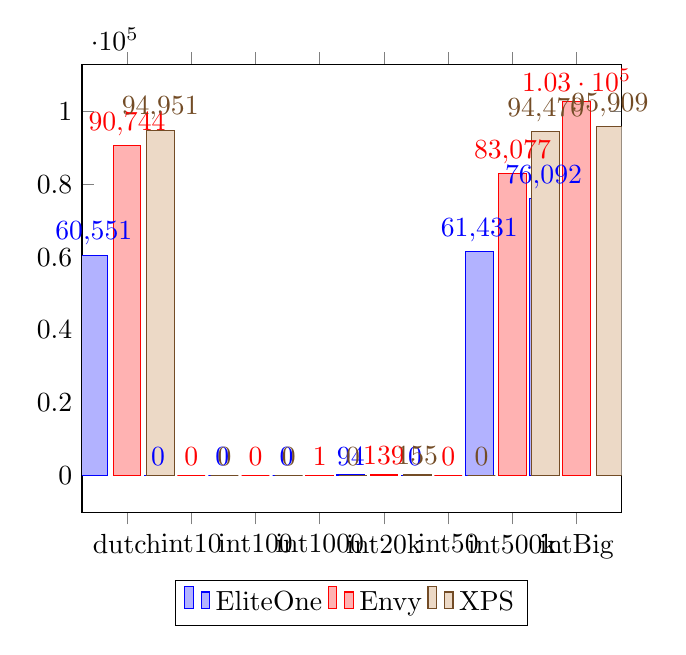
\begin{tikzpicture}
\begin{axis}[
    ybar,
    legend style={at={(0.5,-0.15)},
    anchor=north,legend columns=-1},
    nodes near coords,
    enlargelimits,
    symbolic x coords={dutch, int10, int100, int1000, int20k, int50, int500k, intBig},
    xtick=data]
    \addplot coordinates {
        (dutch, 60551)
        (int10, 0)
        (int100, 0)
        (int1000, 0)
        (int20k, 94)
        (int50, 0)
        (int500k, 61431)
        (intBig, 76092)
    };
    \addplot coordinates {
        (dutch, 90744)
        (int10, 0)
        (int100, 0)
        (int1000, 1)
        (int20k, 139)
        (int50, 0)
        (int500k, 83077)
        (intBig, 102811)
    };
    \addplot coordinates {
        (dutch, 94951)
        (int10, 0)
        (int100, 0)
        (int1000, 0)
        (int20k, 155)
        (int50, 0)
        (int500k, 94470)
        (intBig, 95909)
    };
\legend{EliteOne, Envy, XPS}
\end{axis}
\end{tikzpicture}
\end{center}

%==============================================================================
%% Part 2 : Page 6 (Merge Sort Graph)

\newpage

\subsection{Merge Sort Graph}
Merge Sort is stable and more efficient than Quick Sort for larger arrays. Clearly, sort times are much faster than Basic Quick Sort. \\

\smallskip

\pgfplotsset{width=15cm,compat=1.9}
\begin{center}
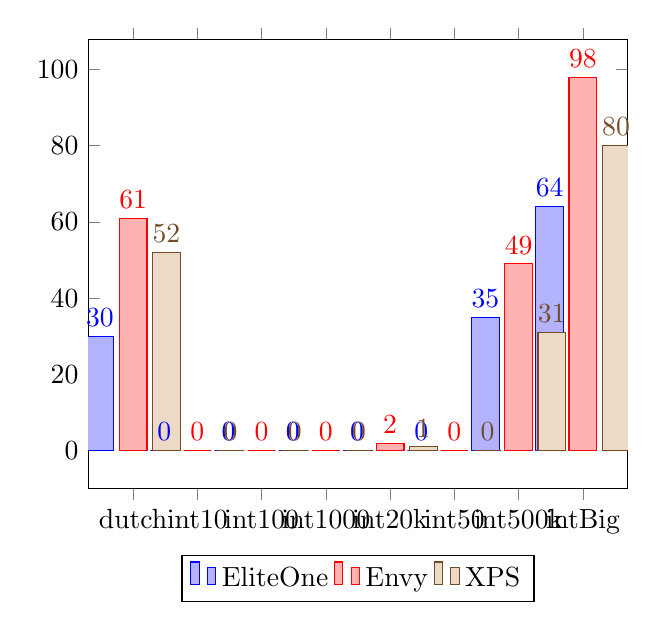
\begin{tikzpicture}
\begin{axis}[
    ybar,
    legend style={at={(0.5,-0.15)},
    anchor=north,legend columns=-1},
    nodes near coords,
    enlargelimits,
    symbolic x coords={dutch, int10, int100, int1000, int20k, int50, int500k, intBig},
    xtick=data]
    \addplot coordinates {
        (dutch, 30)
        (int10, 0)
        (int100, 0)
        (int1000, 0)
        (int20k, 0)
        (int50, 0)
        (int500k, 35)
        (intBig, 64)
    };
    \addplot coordinates {
        (dutch, 61)
        (int10, 0)
        (int100, 0)
        (int1000, 0)
        (int20k, 2)
        (int50, 0)
        (int500k, 49)
        (intBig, 98)
    };
    \addplot coordinates {
        (dutch, 52)
        (int10, 0)
        (int100, 0)
        (int1000, 0)
        (int20k, 1)
        (int50, 0)
        (int500k, 31)
        (intBig, 80)
    };
\legend{EliteOne, Envy, XPS}
\end{axis}
\end{tikzpicture}
\end{center}

%==============================================================================
%% Part 2 : Page 7 (Selection Sort Graph)

\newpage

\subsection{Selection Sort Graph}
The complexity of Selection Sort is O$(n^2)$. The technique is unstable and performs far more comparisons than Insertion Sort. Although \code{dutch.txt} sorts faster, there is variation for \code{int500k.txt} and \code{intBig.txt} across the machines when compared to Insertion Sort Graph. \\

\smallskip

\pgfplotsset{width=15cm,compat=1.9}
\begin{center}
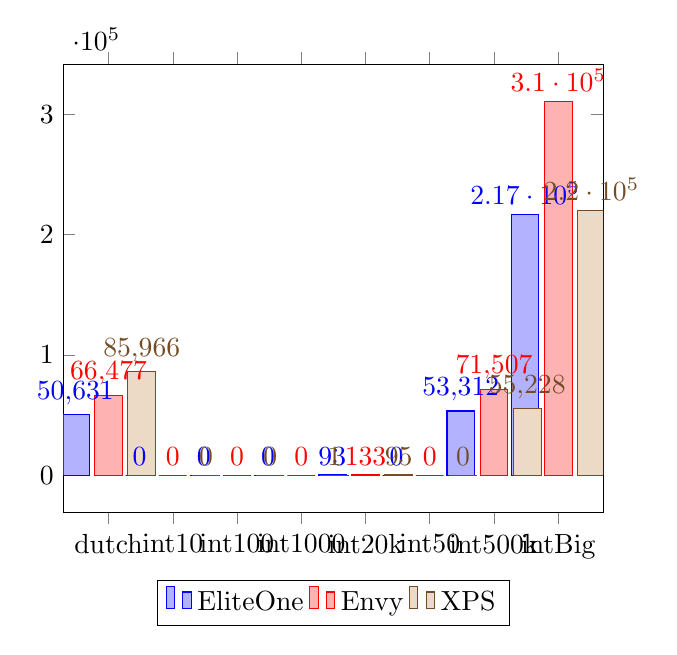
\begin{tikzpicture}
\begin{axis}[
    ybar,
    legend style={at={(0.5,-0.15)},
    anchor=north,legend columns=-1},
    nodes near coords,
    enlargelimits,
    symbolic x coords={dutch, int10, int100, int1000, int20k, int50, int500k, intBig},
    xtick=data]
    \addplot coordinates {
        (dutch, 50631)
        (int10, 0)
        (int100, 0)
        (int1000, 0)
        (int20k, 93)
        (int50, 0)
        (int500k, 53312)
        (intBig, 216915)
    };
    \addplot coordinates {
        (dutch, 66477)
        (int10, 0)
        (int100, 0)
        (int1000, 0)
        (int20k, 133)
        (int50, 0)
        (int500k, 71507)
        (intBig, 310408)
    };
    \addplot coordinates {
        (dutch, 85966)
        (int10, 0)
        (int100, 0)
        (int1000, 1)
        (int20k, 95)
        (int50, 0)
        (int500k, 55228)
        (intBig, 220203)
    };
\legend{EliteOne, Envy, XPS}
\end{axis}
\end{tikzpicture}
\end{center}

%==============================================================================
%% Part 2 : Page 8 (Averages)

\newpage
\newgeometry{top=2.0in,bottom=1.2in}

\subsection{Averages}
Here we have the average times of all techniques considering all machines.\\
Quick Sort (Cutoff) is an average of all cutoffs on Envy.

\vspace{1cm}

\begin{table}[H]
\centering
\begin{tabular}{|c|c|c|c|c|}
\hline
            & Basic Quick Sort & Quick Sort (Cutoff) & Quick Sort (MoT) & 3 Way QS \\ \hline
\code{dutch.txt}   & 330 ms           & 370.25 ms           & 318.67 ms        & 35 ms    \\
\code{int10.txt}   & 0 ms             & 0 ms                & 0 ms             & 0 ms     \\
\code{int100.txt}  & 0 ms             & 0.25 ms             & 0 ms             & 0 ms     \\
\code{int1000.txt} & 0 ms             & 0 ms                & 0 ms             & 0 ms     \\
\code{int20k.txt}  & 1.33 ms          & 1.75 ms             & 2.33 ms          & 1.33 ms  \\
\code{int50.txt}   & 0 ms             & 0 ms                & 0.33 ms          & 0 ms     \\
\code{int500k.txt} & 48 ms            & 50.25 ms            & 43.67 ms         & 39.33 ms \\
\code{intBig.txt}  & 87 ms            & 100 ms              & 88 ms            & 83 ms    \\ \hline
\end{tabular}
\caption{average times (1/2)}
\label{tab:my-table}
\end{table}

\bigskip

\begin{table}[H]
\centering
\begin{tabular}{|c|c|c|c|}
\hline
            & Insertion Sort & Merge Sort & Selection Sort                  \\ \hline
\code{dutch.txt}   & 82,082 ms      & 47.67 ms   & 67,691 ms                       \\
\code{int10.txt}   & 0 ms           & 0 ms       & 0 ms                            \\
\code{int100.txt}  & 0 ms           & 0 ms       & 0 ms                            \\
\code{int1000.txt} & 0.33 ms        & 0 ms       & 0.33 ms                         \\
\code{int20k.txt}  & 129.33 ms      & 1 ms       & 107 ms                          \\
\code{int50.txt}   & 0 ms           & 0 ms       & 0 ms                            \\
\code{int500k.txt} & 79,659 ms      & 38.33 ms   & 60,015 ms                       \\
\code{intBig.txt}  & 91,604 ms      & 80.67 ms   & 2.49 x 10^5 ms                  \\ \hline
\end{tabular}
\caption{average times (2/2)}
\label{tab:my-table}
\end{table}

\restoregeometry

%==============================================================================
%% Part 3

\newpage
\newgeometry{top=1.0in,bottom=1.0in}

\section{Part 3}

\subsection{Running Time}
\begin{itemize}
    \item The cost of partitioning is O$(n)$.
    \item The best case is O$(n$ $log$ $n)$.
    \item The worst case is O$(n^2)$.
\end{itemize}

\subsection{Worst Case}
Quick Sort depends on choosing the right pivot (hence its \textit{instability}) and partitioning the array. The worst case for Quick Sort is when:
\begin{itemize}
    \item there is \textbf{unbalanced} partitioning in each of its binary recursions;
    \item the pivot is the smallest/largest element;
    \item the array is already sorted (increasing/decreasing)
\end{itemize}

\subsection{Pathological.java}
\code{Pathological.java} implements a class with a \code{main(String[] args)} method that will generate pathological input sequences that will require quadratic time to be sorted using Quick Sort with a median-of-three partitioning scheme. It operates as follows:
\begin{enumerate}
    \item \code{generatePathological(int n)} is called with the size of array as parameter.
    \item An ArrayList is filled with \code{n} unique elements.
    \begin{itemize}
        \item \code{n} is unknown, it can be odd or even, so middle element cannot be fiddled with.
    \end{itemize}
    \item Since median-of-three is used, the following were considered:
    \begin{itemize}
        \item 3 elements would be compared and sorted;
        \item all elements must be unique;
        \item therefore, the pivot cannot be the smallest or largest element. Instead, it can be the second smallest / largest element.
    \end{itemize}
    \item The ArrayList is first sorted beforehand, and then the largest and second largest elements are placed at the two ends of the array.
    \item This ArrayList is returned as \code{int[]} (an array of type primitive \code{int}).
\end{enumerate}
\textbf{PS: \code{StackOverFlowError} is sorted by adding \code{-Xmx320m -Xss208m} in Eclipse's\\ Run\textgreater Run Configuration\textgreater Java Application\textgreater Arguments\textgreater VM Arguments}. \\
The following are the times\footnote[1]{Tested on \textbf{EliteOne}} for \code{n} elements:

\begin{table}[H]
\centering
\begin{tabular}{|c|c|}
\hline
                     & Time (ms) \\ \hline
\code{n} = 20,000    & 78                        \\ \hline
\code{n} = 100,000   & 2,140                      \\ \hline
\code{n} = 500,000   & 4,881                     \\ \hline
\code{n} = 1,000,000 & 14,443                          \\ \hline
\end{tabular}
\caption{pathological array sort times}
\label{tab:my-table}
\end{table}

(Since worst case times vary \textbf{a lot}, an \textbf{average of 20} runs for each \code{n} has been taken.)

\restoregeometry

\end{document}